%-------------------------------------------------------------
% Language
% Use the option "language=EN" to set the beamer theme in English. Use
% the option "language=ES" to set the beamer theme in Spanish.

% Colors
% Use the option "color=white" to set the background in white and the
% bottom bar in blue. Use the option "color=blue" to set the
% background in blue and the bottom bar in white. Use the option
% "color=blue2" to set the background in blue and the bottom bar in
% blue.

% Font Color
% Use the option "fontc=black" to set the font color in black. If this
% argument is not given the default color is set depending of the
% color scheme selected.

% Notes:
% Do not use \large inside multicols
% Enumerate require \justifying command
% Tables captions bellow the tabular
% With citations, note = {} may only work for @misc

% Credits: https://github.com/alejogm0520 & Samuel Plazas Escudero
%-------------------------------------------------------------

%--Principal packages
\documentclass[xcolor=table, aspectratio=43,8pt]{beamer} % 4:3; can be 16:9; [...,8pt,t] in order to start text of all frames on the upper part; add: draft to not compile figures.
\usetheme[language=EN, color=white]{EAFIT}
\usepackage[english]{babel}
\usepackage[utf8]{inputenc}

\usepackage{amsmath,amsfonts,amssymb,cancel} % Equations; physics is optional and sometimes problematic!
\usepackage{verbatim} % Environments, \begin{comment}
%--Arial
\usepackage{helvet}\renewcommand{\familydefault}{\sfdefault} % It's ok
%--David Plazas recommended
%\usepackage{libertine} % Normal
%--Carlos Cuartas 
%\usepackage[T1]{fontenc}\usepackage{lmodern} % Best
%--Beamer packages
\usepackage{tikz} % For making vectorized figures, arrows
\usepackage{ifthen} % For specifying conditionals for sections
\usepackage{ragged2e}\justifying % Whole text justified, except enumerate: add \justifying
\usepackage{multicol} % Multiple columns in one frame
%--Tables-Figures


\usepackage{booktabs,multirow} % Bookstyle tables
\usepackage{array} % Custom width and centered
\newcolumntype{P}[1]{>{\centering\arraybackslash}p{#1}} % horizontal centering but use custom width
\newcolumntype{M}[1]{>{\centering\arraybackslash}m{#1}} % horizontal and vertical centering but use custom width
%-Figure label
\usepackage[labelsep=period,justification=justified,format=plain]{caption} % Dot instead of colon and justified caption
%--Figure
\usepackage{graphicx,subcaption} % Figures and subfigures
\usepackage{media9} % video and audio
%-Figure-Table on top
\usepackage{float} % Allows to put H instead of ht
\setbeamertemplate{caption}[numbered] % Numbered captions
%---------TOC
\setbeamertemplate{section in toc}[sections numbered]
\setbeamertemplate{subsection in toc}[subsections numbered]
\setbeamerfont{section in toc}{size=\small}
\setbeamerfont{subsection in toc}{size=\footnotesize}
\setbeamertemplate{subsection in toc}{\leavevmode\leftskip=3.2em\rlap{\hskip-2em\inserttocsectionnumber.\inserttocsubsectionnumber}\inserttocsubsection\par} % Indented subsection
\setcounter{tocdepth}{2} % Toc depth, put 1 for only showing there the sections and 2 to include sections
%---------Cite
\usepackage{bibentry} % Full cite foot
\nobibliography* % Full cite foot
\setbeamertemplate{bibliography item}[triangle]% [online][book][article][triangle][text]; Or: \setbeamertemplate{bibliography item}{\insertbiblabel} 
\usepackage{etoolbox} % Package for using justified bibliography 
\apptocmd{\thebibliography}{\justifying}{}{} % Justified bibliography 
%---------Footnotes
\setbeamercolor{footnote}{fg=white} % Footnote white 
\setbeamercolor{footnote mark}{fg=.} % Takes the color depending on the circumpstance
\setbeamercolor{bibliography entry author}{fg=white} % Allows to have white footnote bibs
\setbeamertemplate{footnote}
{
  \hspace*{-1cm} % Horizontal movement
  \vspace*{-3.12cm} % Vertical movement
  \parbox[c][3.64cm]{10.6cm}{\tiny\noindent\insertfootnotemark\insertfootnotetext} % b: bottom, height: 3.3cm, horizontal length: 10.6cm (max horizontal)
% If there are problems, put \vspace*{-2.87cm} and \parbox[c][3.3cm]
% or \vspace*{-2.88cm} and \parbox[c][3.4cm]
% or \vspace*{-3.05cm} and \parbox[c][3.6cm]
% or \vspace*{-3.12cm} and \parbox[c][3.64cm]
}
\renewcommand{\footnoterule}{\kern -3pt \hrule width \textwidth height 0pt\kern 3pt} % No footnoterule
\usepackage{perpage}\MakePerPage{footnote} % Footnote numbered per frame
\renewcommand{\thefootnote}{\Roman{footnote}} % Roman number in footnote
                                              % Cutom: \fnsymbol{footnote}
%------------------------------------
%---------Numbered Slides and Sections
\setbox0=\hbox{\subsecname\unskip}\ifdim\wd0=0pt\else%
 ~--~\insertsubsectionhead
\fi
%------Numbering section: title in bold, centered and with a line
\newcommand{\numb} 
{
  \setbeamertemplate{frametitle}
  {
    \ifx\insertsubsection\empty % No subsection
         \bfseries\thesection.~\insertframetitle~\color{black}\par\vskip-5pt\hrulefill % \centering
    \else % subsection
         \bfseries\thesection.~\insertframetitle~\color{black}\par\vskip-9pt\hrulefill\par\vskip3pt{\large\thesection.\thesubsection~\insertframesubtitle} % Subsection with smaller size;
    \fi
  }
}
%------No numbering section: title in bold, centered and with a line
\newcommand{\nonumb}
{
  \setbeamertemplate{frametitle}{\bfseries\color{black}\centering\insertframetitle\par\vskip-6pt\hrulefill}
}
%------------------------------------
%--No hyphenation on text
\tolerance=1
\emergencystretch=\maxdimen
\hyphenpenalty=10000
\hbadness=10000
%------------------------
%---------Itemize justified in beamer
\makeatletter
\renewcommand{\itemize}[1][]{
  \beamer@ifempty{#1}{}{\def\beamer@defaultospec{#1}}
  \ifnum \@itemdepth >2\relax\@toodeep\else
    \advance\@itemdepth\@ne
    \beamer@computepref\@itemdepth % Sets \beameritemnestingprefix
    \usebeamerfont{itemize/enumerate \beameritemnestingprefix body}
    \usebeamercolor[fg]{itemize/enumerate \beameritemnestingprefix body}
    \usebeamertemplate{itemize/enumerate \beameritemnestingprefix body begin}
    \list
      {\usebeamertemplate{itemize \beameritemnestingprefix item}}
      {\def\makelabel##1{
          {
            \hss\llap{{
                \usebeamerfont*{itemize \beameritemnestingprefix item}
                \usebeamercolor[fg]{itemize \beameritemnestingprefix item}##1}}
          }
        }
      }
  \fi
  \beamer@cramped
  \justifying % Justified itemize
  \beamer@firstlineitemizeunskip
}
\makeatother
%------------------------
%---------get current section name for showing it at its begining
\usepackage{nameref}
\makeatletter
\newcommand*{\currentname}{\@currentlabelname}
\makeatother
%---------Shows in which section we are at the begining of each one
\begin{comment}
\AtBeginSection[]
{
\begin{frame}[plain,noframenumbering]
  \begin{beamercolorbox}[ht=\paperheight,wd=\paperwidth, center]{Portada}
    \begin{center}\textbf{\LARGE \currentname}\end{center} % Leave the next space mandatorily

    \vspace{0.44\paperheight}
  \end{beamercolorbox}
\end{frame}
}
\end{comment}
%-------------------(CONSTANTLY BEING EDITED)------------------
%---------TEXTBLOCKS-GRID 
\usepackage[absolute,overlay,showboxes]{textpos}
%\usepackage[texcoord,grid,gridunit=mm,gridcolor=red!10,subgridcolor=green!10]{eso-pic} % Helping grids, comment when publishing
%---------NOTES IN BEAMER
\AtBeginNote{\Huge}\newcommand{\notei}[1]{\note[item]{\Huge{\textcolor{blue}{#1}}}} % Use \notei{text} everywhere % [1] means one parameter located in #1 (input). 
\setbeamertemplate{note page}[plain] % Plain style for notes page
\setbeameroption{show notes} % {show notes} or {hide notes}
% \setbeameroption{show notes on second screen=right}
% as well you can use \documentclass[notes=only] at the beginning of the code
%-----------More elaborated notes
%\setbeamercolor{note page}{bg=white!90!black, fg=black}
%\setbeamercolor{note title}{bg=white!30!red, fg=black}
%\setbeamercolor{note date}{parent=note title}
%---------Itemize, enumberate and lists inside them
%\setbeamertemplate{itemize/enumerate body begin}{\LARGE} % Body
\setbeamertemplate{itemize/enumerate subbody begin}{\Large} % Subbody
%---------COLOR DEFINITIONS
\definecolor{azure(colorwheel)}{rgb}{0.0, 0.5, 1.0} % Define colors here
\definecolor{blue(ryb)}{rgb}{0.01, 0.28, 1.0}

\usepackage[normalem]{ulem}
\useunder{\uline}{\ul}{}

\usepackage{url}

\usepackage{mathtools}
\DeclarePairedDelimiter{\ceil}{\lceil}{\rceil}
%%%%%%%%%%%%%%%%%%%%%%%
%Start of the Document%
%%%%%%%%%%%%%%%%%%%%%%%

%---------COVER PAGE
  \title{INTRODUCTION TO NUMERICAL SOLUTION \\[1ex]OF FRACTIONAL SYSTEMS}
\author{\normalfont\texorpdfstring{Presented by:\\Mateo Restrepo S.\\Juan S. Cárdenas R. \\David Plazas E.\\Juan J. Jaramillo C. \\[1ex]Prof.:\\ Samir Posada M.}{}}

\def\eafit{EAFIT University}
\def\materia{Numerical Analyisis}
\def\fecha{2019}

\begin{document}
\nonumb
\begin{frame}
% Portada Inspira Crea Transforma
\end{frame}
%%%%%%%%%%%%%%%%%%%%%%%%%%%%%%%%%%%%%%%%%%%%%%%%%%%%%%%%%%%%%%%%%%%%%%%%%%%%
\begin{frame}
\begin{center}
  \titlepage % Cover page
\end{center}
\end{frame}
%%%%%%%%%%%%%%%%%%%%%%%%%%%%%%%%%%%%%%%%%%%%%%%%%%%%%%%%%%%%%%%%%%%%%%%%%%%%
\begin{frame}{CONTENIDO}
\begin{multicols}{2}
  \tableofcontents
\end{multicols}
\end{frame}
\numb

\section{INTRODUCTION}
\subsection{Fractional Derivatives}
\begin{frame}{INTRODUCTION}
\framesubtitle{Fractional Derivatives}
\begin{multicols}{2}
    \textbf{Pros}
    \begin{itemize}
        \item Generalization of ordinary derivatives.
        \item Nonlocal operators $\longrightarrow$ Memory and heritage.
        \item More accuracy and robustness.
        \item Unexplored areas and applications.
    \end{itemize}
    \columnbreak
    \textbf{Cons}
    \begin{itemize}
        \item There are multiple fractional derivatives definitions.
        \item The derivatives are not always in terms of elementary functions.
        \item Some definitions require strong conditions on the functions to differentiate.
    \end{itemize}
    \end{multicols}
\end{frame}

\subsection{Caputo Definition}
\begin{frame}{INTRODUCTION}
\framesubtitle{Caputo Definition}
The Caputo definition of fractional derivative is
\begin{equation}
    \mathcal{D}_C^\alpha y(t) = J^{m-\alpha}y^{(m)}(t) = \dfrac{1}{\Gamma(m-\alpha)}\int_0^t \dfrac{y^{(m)}(\lambda)}{(t-\lambda)^{1-m+\alpha}}d\lambda
\end{equation}
where $\alpha\geq0$, $m=\ceil{\alpha}$, $\Gamma(\cdot)$ is the gamma function and $J^{m-\alpha}$ is the Riemann-Liouville integral. From now on, the Caputo-type fractional derivative will be denoted as
\begin{equation}
    \mathcal{D}_C^\alpha y(t)=\dfrac{d^\alpha}{dt^\alpha}y(t)
\end{equation}
For example
    \begin{align*}
        \dfrac{d^{0.5}}{dt^{0.5}} [t]&= \dfrac{1}{\Gamma(1-0.5)}\int_0^t \dfrac{d}{d\lambda}(\lambda)\cdot\dfrac{d\lambda}{(t-\lambda)^{1-0.5+1}}\\
      &= \dfrac{1}{\sqrt{\pi}}\int_0^t \dfrac{d\lambda}{(t-\lambda)^{1/2}}\quad\text{, let $u=t-\lambda$ $\rightarrow$ $du=-d\lambda$.}\\
      &= \dfrac{1}{\sqrt{\pi}}\int_0^t \dfrac{du}{u^{1/2}}\\
      &=2\sqrt{\dfrac{t}{\pi}}
    \end{align*}
\end{frame}

\subsection{Riemann-Liouville Integral}
\begin{frame}{INTRODUCTION}
\framesubtitle{Riemann-Liouville Integral}
The Riemann-Liouville integral of order $\alpha$ is defined as
\begin{equation}
    J^\alpha y(t) = \dfrac{1}{\Gamma(\alpha)}\int_{0}^{t}\dfrac{y(\lambda)}{(t-\lambda)^{1-\alpha}}d\lambda
\end{equation}
\textbf{Properties}\\\vspace{0.5cm}
\begin{itemize}
    \item
    \begin{equation}
        J^{\alpha}\left[f(t)+g(t)\right]=J^\alpha f(t)+J^\alpha g(t)
    \end{equation}
    \item \begin{equation}
        J^\alpha J^\beta f(t) = J^{\alpha+\beta} f(t)
    \end{equation}
    \item \begin{equation}
        \dfrac{d^\alpha}{dt^\alpha}\left[ J^\alpha y(t)\right] = y(t)
    \end{equation}
    \item \begin{equation}
            J^\alpha \left[ \dfrac{d^\alpha}{dt^\alpha}y(t)\right] = y(t) - \sum_{r=0}^{m-1}\dfrac{y_rt^r}{r!}
        \end{equation}
\end{itemize}
\end{frame}


\subsection{The Tautochrone Problem}
\begin{frame}{INTRODUCTION}
    \framesubtitle{The Tautochrone Problem}
    It is desired to find a curve such that, if an object starts on any point along this curve, the time that it requires to slide down to the origin is the same.
    
    \begin{multicols}{2}
    \begin{itemize}
        \item Tauto $\rightarrow$ equal.
        \item Chrono $\rightarrow$ time.
        \item Abel, XVIII century.
    \end{itemize}
    Assumptions:
    \begin{itemize}
        \item The object moves only by the force of gravity.
        \item It moves without friction.
    \end{itemize}
    \columnbreak
    \begin{figure}[H]
        \centering
        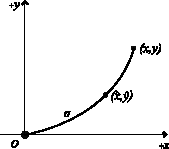
\includegraphics[scale=1.25]{files/taut.pdf}
        \caption{Tautochrone problem.}
    \end{figure}
    
    \end{multicols}
    \begin{center}
    \href{run:gify.gif}{Click for GIF}
    \end{center}
    
\end{frame}


\begin{frame}{INTRODUCTION}
\begin{multicols}{2}
    \framesubtitle{The Tautochrone Problem}
    Using the energy conservation law,
    \begin{align*}
         mgy =& \dfrac{1}{2}m\left(\dfrac{d\sigma}{dt}\right)^2 + mg\hat{y}\\
         \vdots\\
        \dfrac{d^{0.5}}{dy^{0.5}} \sigma ( y ) &= \frac { \sqrt { 2 g } } { \Gamma \left( \frac { 1 } { 2 } \right) } T
    \end{align*}
    Through some analytical procedures, we obtain
    \begin{align*}
        x &= \dfrac{gT^2}{\pi^2}[t+\sin(t)]\\
        y &= \dfrac{gT^2}{\pi^2}[1-\cos(t)]
    \end{align*}
    
    \columnbreak
    \begin{figure}[H]
        \centering
        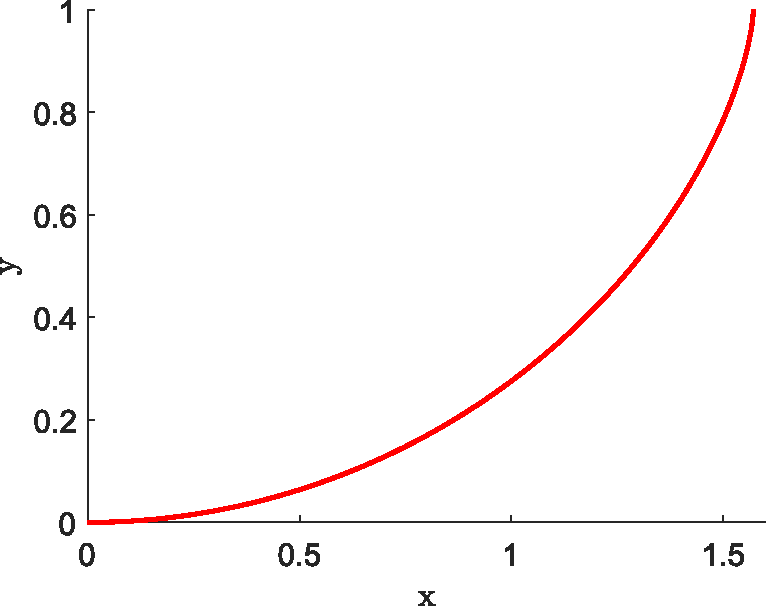
\includegraphics[scale=0.4]{files/tautochrone.pdf}
        \caption{Tautochrone curve.}
        \label{fig:my_label}
    \end{figure}
    \end{multicols}
\end{frame}
\section{INTEGER ORDER METHODS}
\begin{frame}{INTEGER ORDER METHODS}
    The following initial value problem (IVP) will be treated:
    \begin{equation}
        \begin{cases}
        y'=f\left(t,y\right)&
        \\y(0)=y_0\,,\quad t\in[0,T]&
        \end{cases}
    \end{equation}
    \begin{multicols}{2}
    Example:
    \begin{equation}\label{eq:pvi_ex1}
        \begin{cases}
            y'-y=0&\\
            y(0)=-3&
        \end{cases}
    \end{equation}
    The exact solution to this problem is given by
    \begin{equation}
        y(t)=-3e^{-t}
    \end{equation}
    
    \columnbreak
    \begin{figure}[H]
        \centering
        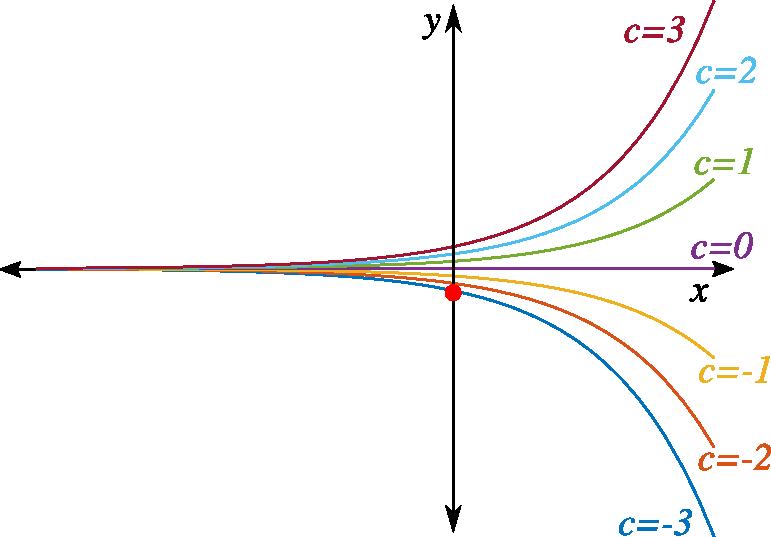
\includegraphics[scale=0.4]{files/ex_ivp_1.pdf}
        \caption{Solution for problem \ref{eq:pvi_ex1}.}
    \end{figure}
    \end{multicols}
\end{frame}



\subsection{Fourth-Order Runge-Kutta Method (RK4)}
\begin{frame}{INTEGER ORDER METHODS}
    \framesubtitle{Fourth-Order Runge-Kutta Method (RK4)}
    \begin{itemize}
        \item Improved Euler with more accuracy.
        \item $4^{th} order$ $\rightarrow$ optimal.
    \end{itemize}
    This method approximates the solution to the IVP as follows:
    
    \begin{equation}
        \begin{split}
            y_{i+1}=y_i+h\left(\dfrac{k_1+2k_2+2k_3+k_4}{6}\right)
        \end{split}
    \end{equation}
    where
    \begin{multicols}{2}
    \begin{equation*}
    \begin{array} { l } { k _ { 1 } = f \left( t _ { i } , y _ { i } \right) } \\
    { k _ { 2 } = f \left( t _ { i } + h / 2 , y _ { i } + h k _ { 1 } / 2 \right) } \\
    { k _ { 3 } = f \left( t _ { i } + h / 2 , y _ { i } + h k _ { 2 } / 2 \right) } \\ 
    { k _ { 4 } = f \left( t _ { i } + h , y _ { i } + h k _ { 3 } \right) } \end{array}
\end{equation*}
The algorithm works as
\begin{center}
    \texttt{y = runge\_kutta(f,y0,T,N)}
\end{center}
\columnbreak
\begin{figure}[H]
    \centering
    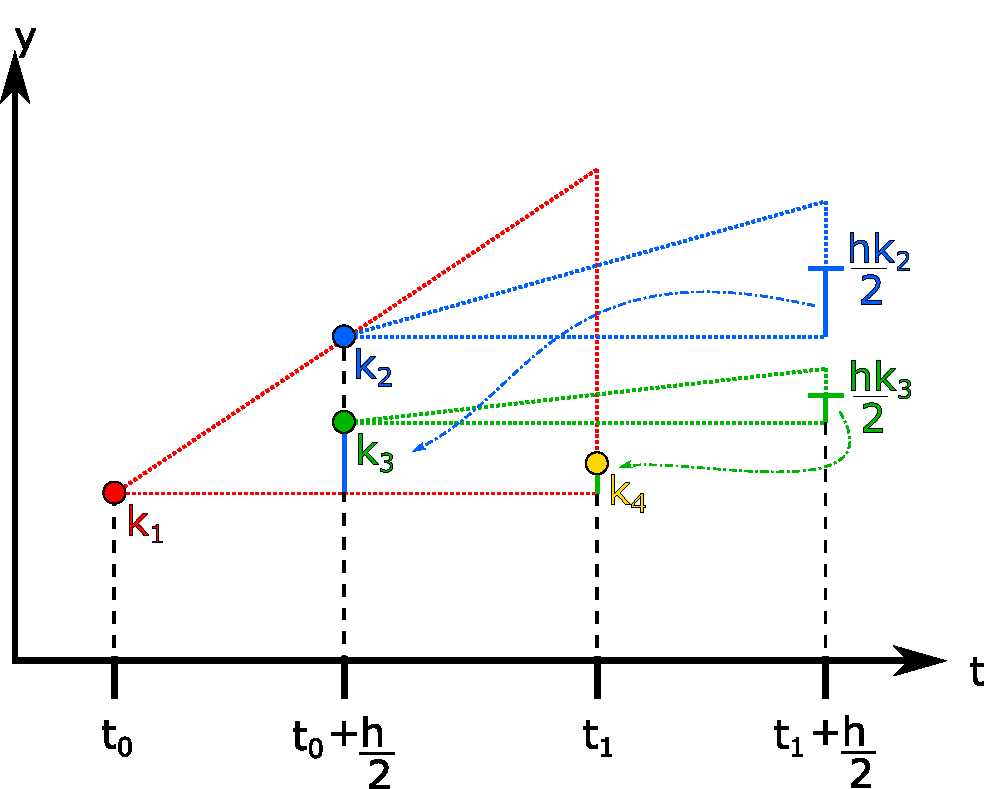
\includegraphics[scale=0.275]{files/sv.pdf}
\end{figure}
\end{multicols}


\end{frame}

\subsection{Comparison Euler - RK4}
\begin{frame}{INTEGER ORDER METHODS}
    \framesubtitle{Comparison Euler - RK4}
    \textbf{Example: approximate a solution to the IVP} 
    \begin{equation}
    \begin{cases}
        y' = 10e^{-\frac{(t-2)^2}{2}}\left(10\cos(10t)-(t-2)\sin(10t)\right)&\\ 
        y(0) = 0&
    \end{cases}
    \end{equation}
The exact solution to this problem is
\begin{equation}
    y(t) = 10e^{-\frac{(t-2)^2}{2}}\sin(10t)
\end{equation}
\begin{multicols}{2}
$\qquad\quad$\textbf{Euler}\begin{figure}[H]
        \centering
        \only<1>{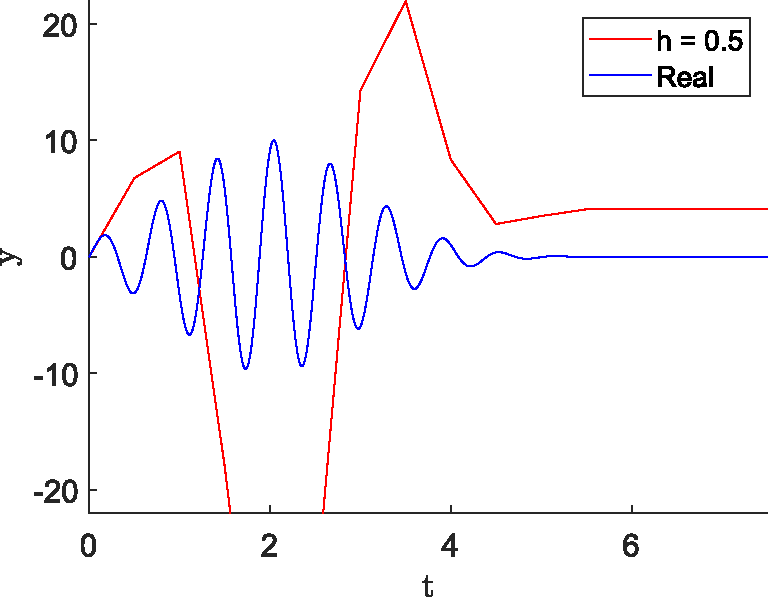
\includegraphics[scale=0.35]{files/rk4vsEuler/euler_05.pdf}}
        \only<2>{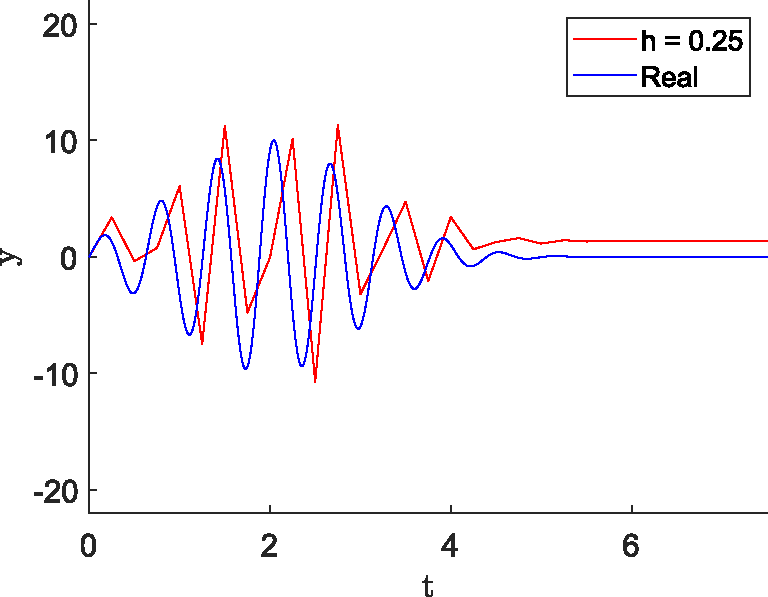
\includegraphics[scale=0.35]{files/rk4vsEuler/euler_025.pdf}}
        \only<3>{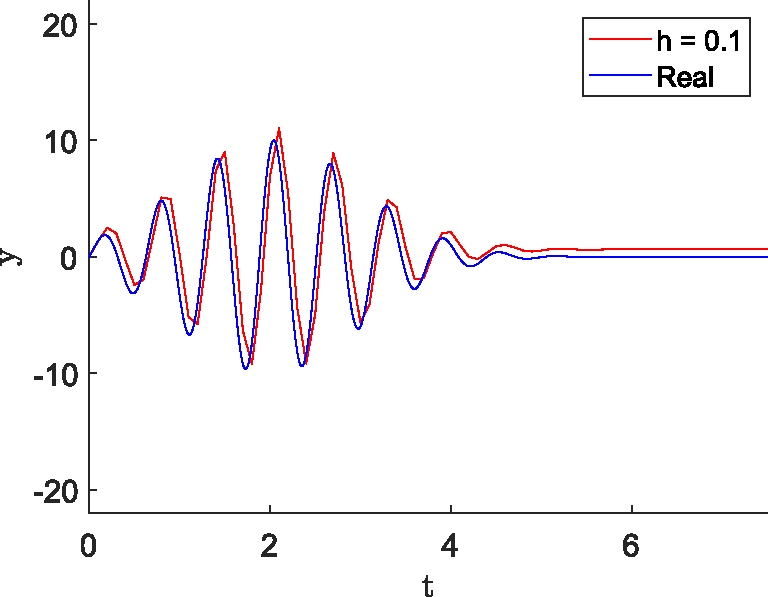
\includegraphics[scale=0.35]{files/rk4vsEuler/euler_01.pdf}}
        \only<4>{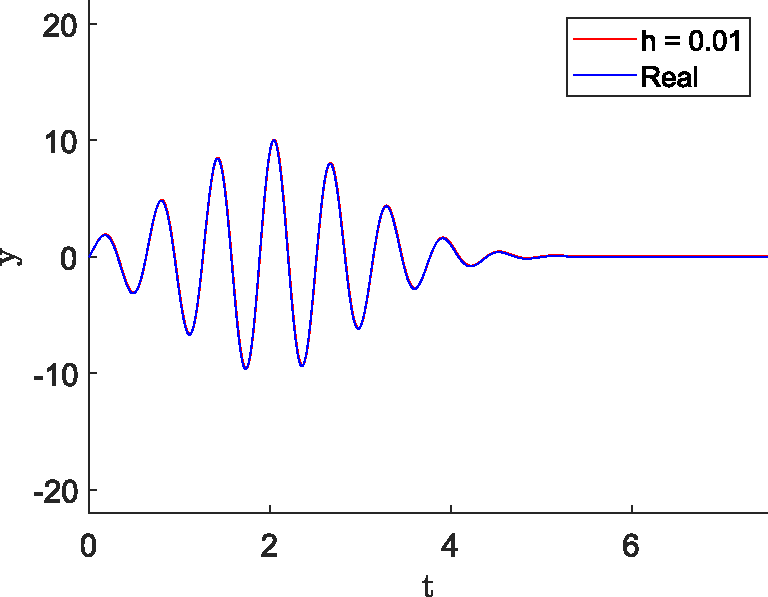
\includegraphics[scale=0.35]{files/rk4vsEuler/euler_001.pdf}}
    \end{figure}\columnbreak$\quad\qquad$\textbf{RK4}
    \vspace{-0.5cm}\begin{figure}[H]
        \centering
        \only<1>{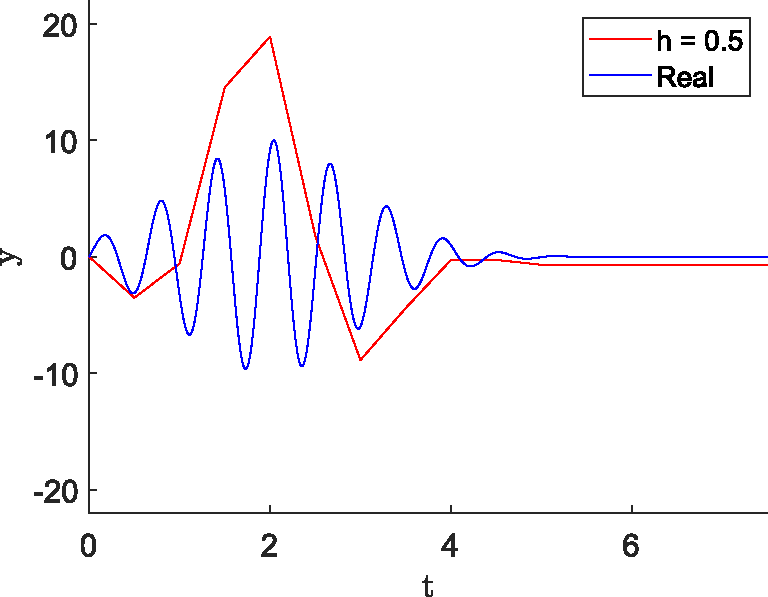
\includegraphics[scale=0.325]{files/rk4vsEuler/rk4_05.pdf}}
        \only<2>{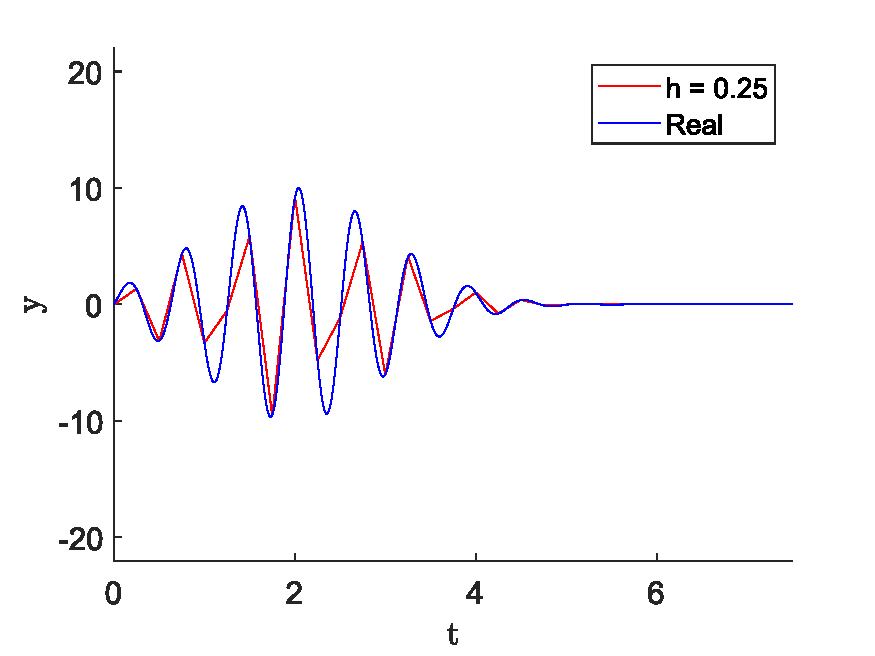
\includegraphics[scale=0.325]{files/rk4vsEuler/rk4_025.pdf}}
        \only<3>{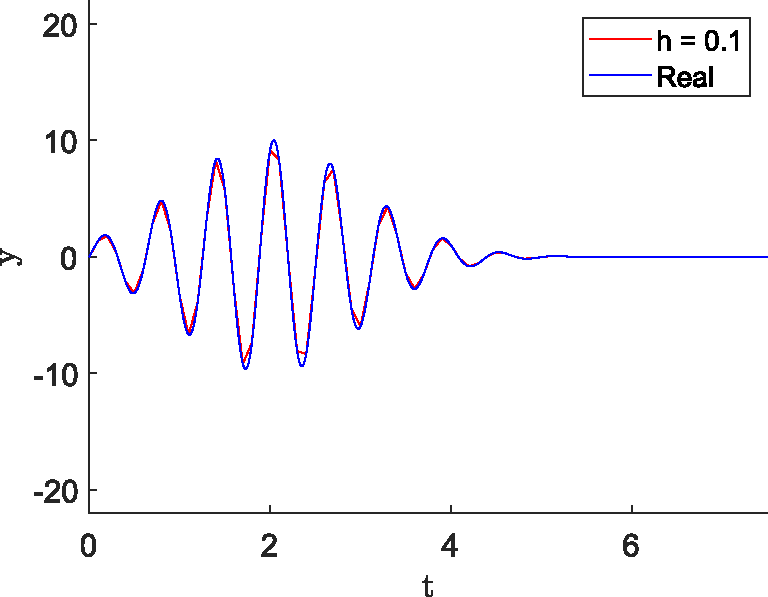
\includegraphics[scale=0.35]{files/rk4vsEuler/rk_01.pdf}}
        \only<4>{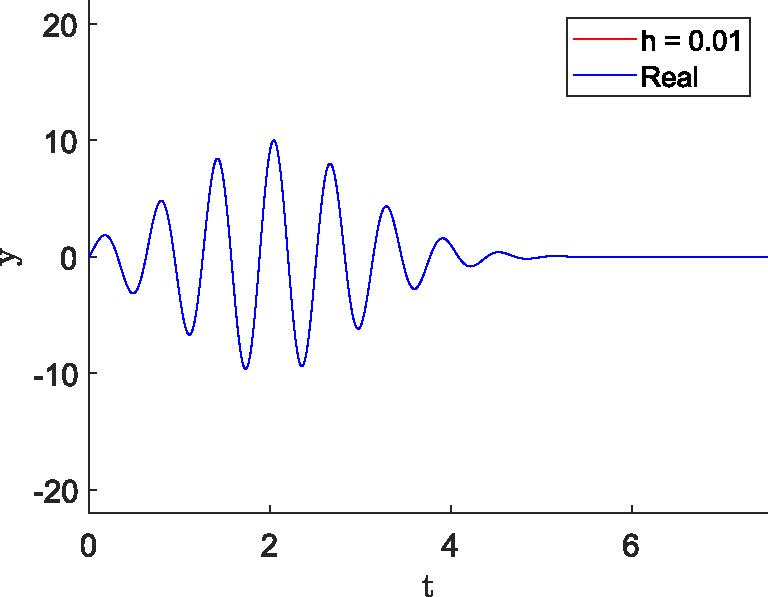
\includegraphics[scale=0.35]{files/rk4vsEuler/rk_001.pdf}}
    
    \end{figure}
\end{multicols}
\end{frame}

\subsection{Systems of ODEs}
\begin{frame}{INTEGER ORDER METHODS}
    \framesubtitle{Systems of ODEs}
    Consider the system of ordinary differential equations
    \begin{equation}
        \begin{cases}
            y_1'=f_1(t,y_1,\,y_2,\,\dots,\,y_n)&y_1(0)=y_{1}\\ y_2'=f_2(t,y_1,\,y_2,\,\dots,\,y_n)&y_2(0)=y_{2}\\
            \qquad\vdots&\\
            y_n'=f_n(t,y_1,\,y_2,\,\dots,\,y_n)&y_n(0)=y_{n}
        \end{cases}
    \end{equation}
    which can be synthesized as 
    \begin{equation}
        \begin{cases}
            \mathbf{y}'=F(t,\mathbf{y})&\\
            \mathbf{y}(0)=\mathbf{y}_0
        \end{cases}
    \end{equation}
    For example, the Lotka-Volterra equations (predator-prey model) is a system of ODEs as follows:
\begin{equation}
    \begin{cases}{y_1'=\alpha y_1-\beta y_1 y_2}& \\ {y_2'=\delta y_1 y_2-\gamma y_2}&\end{cases}
\end{equation}
where $y_1$ represents the number of preys and $y_2$ is the amount of predators.

\end{frame}

\begin{frame}{INTEGER ORDER METHODS}
    \framesubtitle{Systems of ODEs}
\begin{equation}
    \begin{cases}{y_1'=\alpha y_1-\beta y_1 y_2}& \\ {y_2'=\delta y_1 y_2-\gamma y_2}&\end{cases}
\end{equation}
\begin{figure}[H]
    \centering
    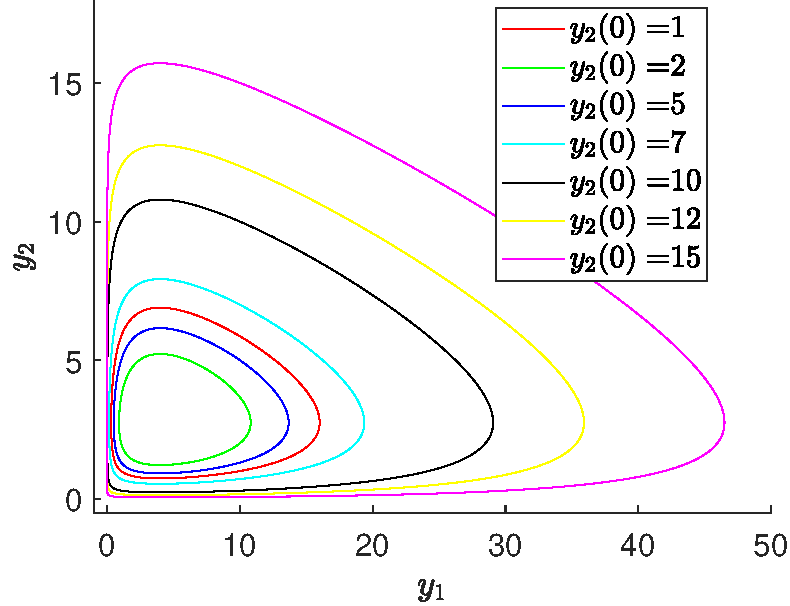
\includegraphics[scale=0.4]{files/Prey.pdf}
    \caption{Phase portrait of Lotka-Volterra equations.}
    \label{fig:lotka}
\end{figure}

\end{frame}

\subsection{Multi-Term ODEs}
\begin{frame}{INTEGER ORDER METHODS}
    \framesubtitle{Multi-Term ODEs}
    In case of higher order ODEs, they can be transformed into a system of first order ODEs, using phase variables $x_i$. Suppose we have an equation as the following:
    \begin{equation}\label{eq:generalDiff}
    \begin{cases}
    y^{(n)}=f\left(t,y,y',...,y^{(n-1)}\right)&\\
    y(0)=y_0,\,\dots,\,y^{(n - 1)}(0)= y_{(n - 1)},\,\,t\in[0,T]&
    \end{cases}
    \end{equation}
    with the following substitution
    \begin{equation}
    \begin{cases}
        x_1 = y&\\
        x_2 = y'&\\
        \qquad\vdots&\\
        x_n = y^{(n-1)}&
    \end{cases}\longrightarrow\begin{cases}
        x_1'=x_2&\\
        x_2'=x_3&\\
        \qquad\vdots&\\
        x_{n-1}'=x_n&\\
        x_n'=f\left(t,x_1,x_2,...,x_{n-1},x_n\right)
    \end{cases}
\end{equation}
\begin{equation*}
    x_1(0)=y_0,\dots,\,x_{n - 1}(0)= y_{(n - 1)}
\end{equation*}

\end{frame}

\begin{frame}{INTEGER ORDER METHODS}
    \framesubtitle{Multi-Term ODEs}
    Example: consider the Duffing oscillator (\href{run:Spring_pendulum.gif}{Click for GIF})
    \begin{equation}
        y''+\delta y'+\alpha y+\beta y^{3}=\gamma \cos (\omega t)
    \end{equation}
    the equivalent system of first order ODEs is
    \begin{equation}
        \begin{cases}
        x_1 = y&\\
        x_2 = y'&\\
    \end{cases}\longrightarrow
    \begin{cases}
        x_1'=x_2&\\
        x_2'=-\delta x_2-\alpha x_1-\beta x_1^3 + \gamma\cos(\omega t)
    \end{cases}
    \end{equation}
    \begin{multicols}{2}
        \begin{figure}[H]
            \centering
            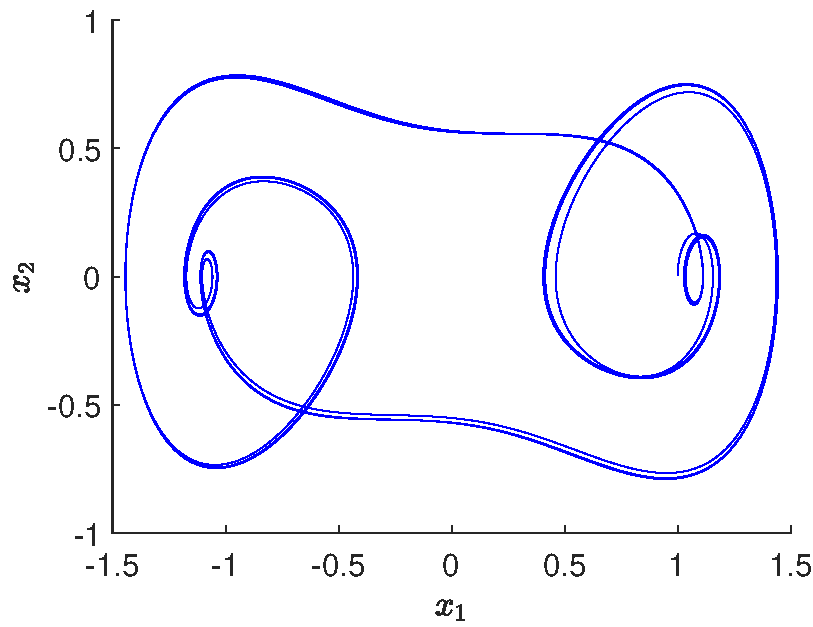
\includegraphics[scale=0.34]{files/Phase.pdf}
        \end{figure}
        \columnbreak
        \begin{figure}[H]
            \centering
            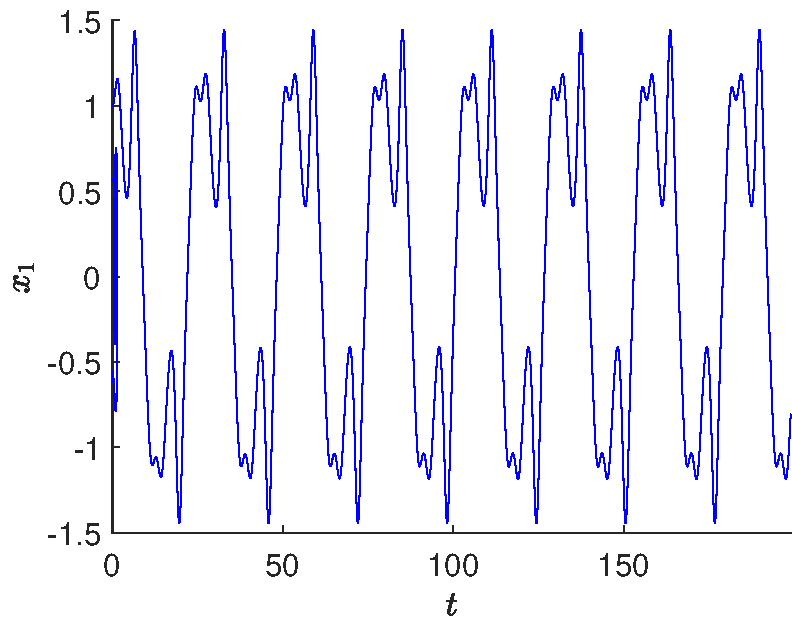
\includegraphics[scale=0.34]{files/Time.pdf}
        \end{figure}
    \end{multicols}
    $\delta=0.3$, $\alpha =-1$, $\beta=1$,$\gamma=0.37$, $\omega =1.2$ and initial conditions $x_1(0)=1$,  $x_2(0)=0$.
\end{frame}


%%%%%%%%%%%% fraccional %%%%%%%%%%

\section{FRACTIONAL ORDER METHODS}
\begin{frame}{FRACTIONAL ORDER METHODS}
Consider the fractional IVP
\begin{equation}\label{eq:frac_dif}
     \begin{cases}
     \dfrac{d^ { \alpha }}{dt^{\alpha }}y(t) = f(t,y)&\\ y(0)=y_0,\,\dots,y^{(m-1)}(0)= y_{(m-1)}\quad \alpha \in \mathbb{R}^+\quad t\in[0,T]&
     \end{cases}
\end{equation}
\begin{multicols}{2}
where $m=\ceil{\alpha}$. \\[0.4cm]\textbf{Example}
\begin{equation}
    \dfrac{d^{0.5}}{dt^{0.5}} y(t)=2\sqrt{\dfrac{y}{\pi}}
\end{equation}
whose solution is \begin{equation}
    y(t)=t
\end{equation}
\columnbreak
\begin{figure}
    \centering
    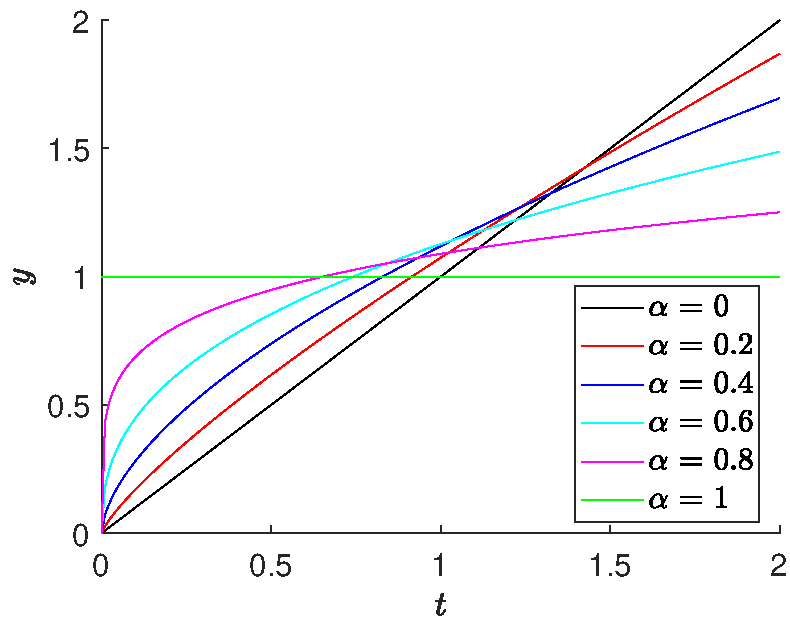
\includegraphics[scale=0.4]{files/t_derivative.pdf}
\end{figure}
\end{multicols}
\end{frame}


\subsection{Adams-Bashforth-Moulton Predictor-Corrector (ABM)}
\begin{frame}{FRACTIONAL ORDER METHODS}
\framesubtitle{Adams-Bashforth-Moulton Predictor-Corrector (ABM)}
Using quadrature theory, the solution can be approximated as
\begin{equation}
    \begin{aligned} y _ { h } \left( t _ { n + 1 } \right) =  \sum _ { k = 0 } ^ { [ \alpha ] - 1 } \frac { t _ { n + 1 } ^ { k } } { k ! } y _ { 0 } ^ { ( k ) } + \frac { h ^ { \alpha } } { \Gamma ( \alpha + 2 ) } f \left( t _ { n + 1 } , y _ { h } ^ { \mathrm { p } } \left( t _ { n + 1 } \right) \right) + \frac { h ^ { \alpha } } { \Gamma ( \alpha + 2 ) } \sum _ { j = 0 } ^ { n } a _ { j , n + 1 } f \left( t _ { j } , y _ { h } \left( t _ { j } \right) \right) \end{aligned}
\end{equation}
\begin{itemize}
    \item $y _ { h } ^ { \mathrm { p } } \left( t _ { n + 1 } \right)$ is a predicted value.
    \item $a _ { j , n + 1 }$ is a quadrature coefficient.
\end{itemize}
The algorithm works as
\begin{center}
    \texttt{y = abm(f,alpha,y0,T,N)}
\end{center}
\begin{itemize}
    \item \texttt{f} is the right-hand side of the differential equation.
    \item \texttt{alpha} is the order of the differential equation.
    \item \texttt{y0} is the initial conditions.
    \item \texttt{T} is the simulation time.
    \item \texttt{N} is the number of partitions on the interval $[0,\text{\texttt{T}}]$.
\end{itemize}
\end{frame}

\begin{frame}{FRACTIONAL ORDER METHODS}
\framesubtitle{Adams-Bashforth-Moulton Predictor-Corrector (ABM)}
\textbf{Example}\\\vspace{0.5cm}
Give an approximate solution to
\begin{equation}
    \begin{cases}
        \dfrac{d^{1.25}}{dt^{1.25}}y(t)=-y(t)&\\
        y'(0)=0,\,y(0)=1
    \end{cases}
\end{equation}

\begin{multicols}{2}
\null \vfill
The exact solution is given by

\begin{equation}
    y(t) = E_{1.25,\,1}(-t^{1.25})=\sum_{k=0}^{\infty}\dfrac{(-1)^kt^{1.25k}}{\Gamma(1.25k +1)}
\end{equation}
\null \vfill
\columnbreak
\begin{figure}[H]
        \centering
        \only<1>{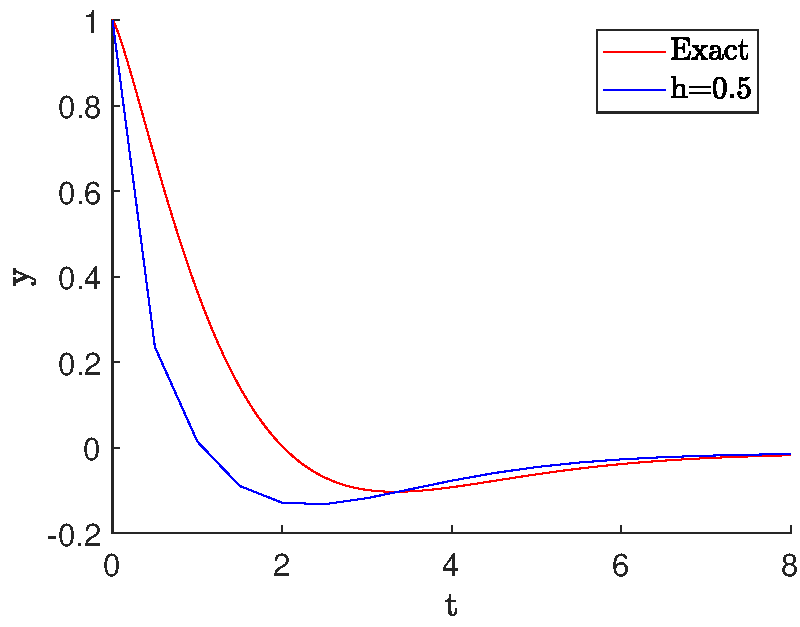
\includegraphics[scale=0.35]{files/comparFrac/ABM_05.pdf}}
        \only<2>{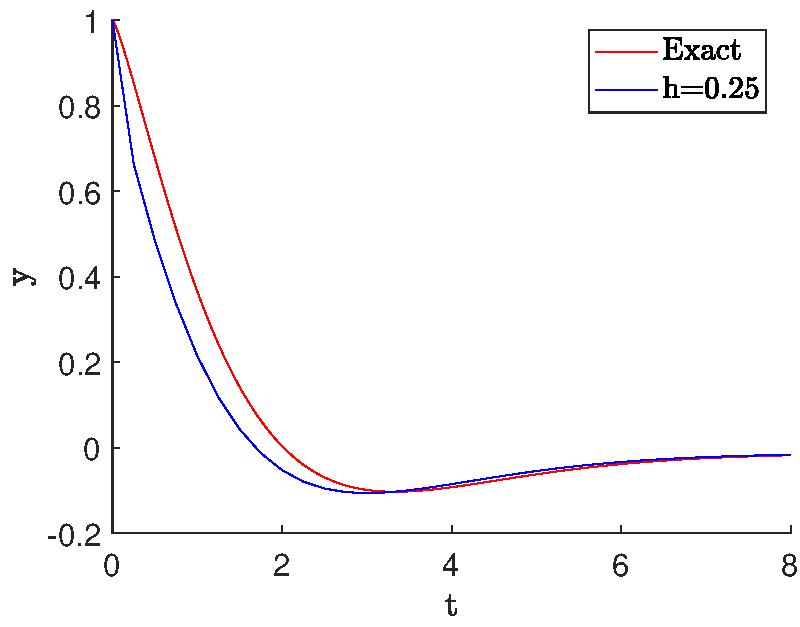
\includegraphics[scale=0.35]{files/comparFrac/ABM_025.pdf}}
        \only<3>{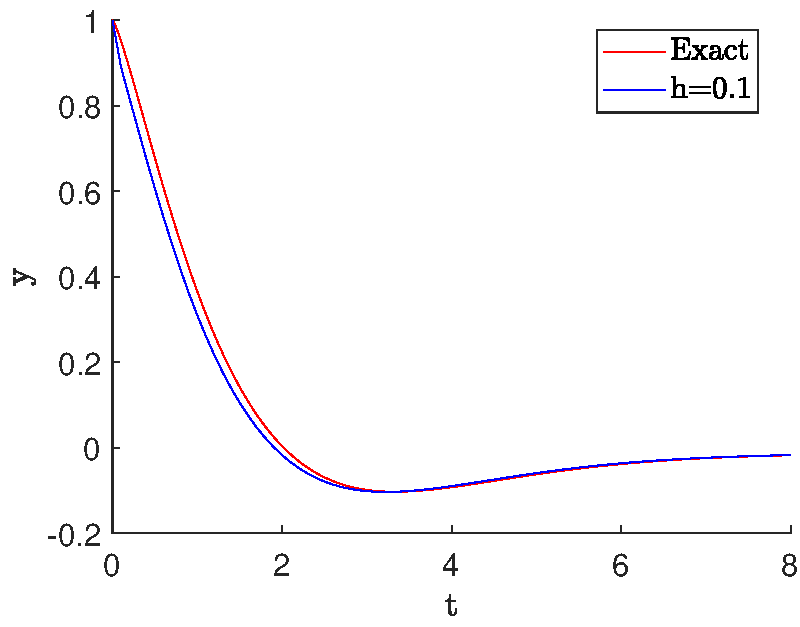
\includegraphics[scale=0.35]{files/comparFrac/ABM_01.pdf}}
        \only<4>{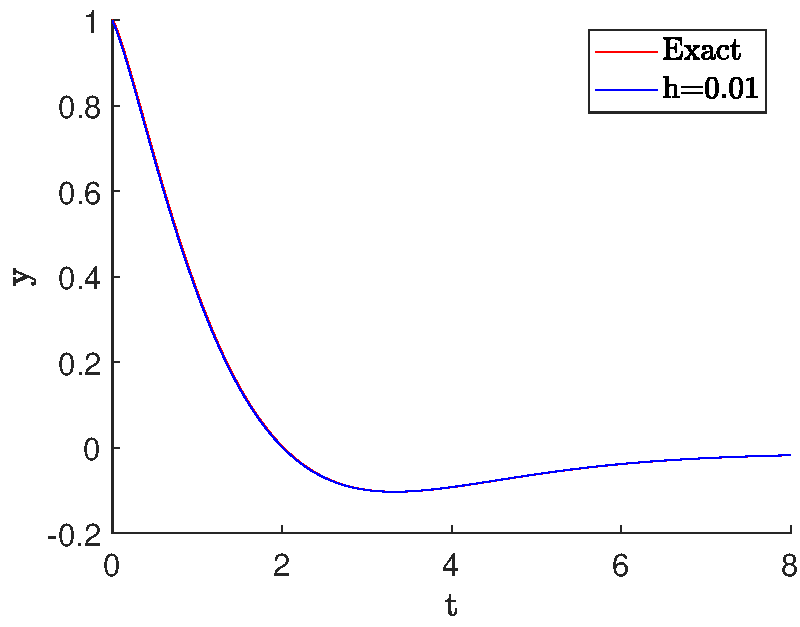
\includegraphics[scale=0.35]{files/comparFrac/ABM_001.pdf}}
    \end{figure}
    \end{multicols}
\end{frame}


\subsection{Decomposition Method}
\begin{frame}{FRACTIONAL ORDER METHODS}
\framesubtitle{Decomposition Method}
Based on decomposing $f$ as follows
    \begin{equation}
        f(t,\mathbf{y})=g(t)+\mathbf{Ay}+h(t,\mathbf{y})
    \end{equation}
Applying the inverse operation to the Caputo fractional derivative
\begin{equation}
    \mathbf{y}(t) = \sum_{r=0}^{m-1}\dfrac{\mathbf{y}_{r}t^r}{r!}+ J^\alpha g(t)+J^\alpha\mathbf{Ay}+J^\alpha h(t,\mathbf{y})
\end{equation}
and supposing a solution in series, we obtain the recursive scheme
\begin{equation}
    \begin{split}
        \mathbf{x}_0&=\sum_{r=0}^{m-1}\dfrac{\mathbf{y}_{r}t^r}{r!}+J^\alpha g(t)\\
        \mathbf{x}_{k+1}&=J^\alpha \mathbf{Ax}_k+J^\alpha \tilde{h}_k\left(t,\sum_{r=0}^k\mathbf{x}_j(t)\right)
    \end{split}
\end{equation}
Where $\tilde{h}_k$ is the Adomian polynomial
\begin{equation}
    \tilde{h}_k\left(t,\sum_{r=0}^{k}\mathbf{x}_j(t)\right)=\dfrac{1}{k!}\left[\dfrac{d^k}{d\lambda^k}h\left(t,\sum_{j=0}^{k}\lambda^j\mathbf{x}_j(t)\right)\Bigg|_{\lambda=0}\right]
\end{equation}
\end{frame}

\begin{frame}{FRACTIONAL ORDER METHODS}
\framesubtitle{Decomposition Method}
The algorithm works as
\begin{center}
    \texttt{ySim = decomposition(f,alpha,y0,N)}
\end{center}
    \textbf{Example}\\\vspace{0.5cm}
Give an approximate solution to
\begin{equation}
    \begin{cases}
        \dfrac{d^{1.25}}{dt^{1.25}}y(t)=-y(t)&\\
        y'(0)=0,\,y(0)=1
    \end{cases}
\end{equation}

\begin{multicols}{2}
\null \vfill
The exact solution is given by

\begin{equation}
    y(t) = E_{1.25,\,1}(-t^{1.25})=\sum_{k=0}^{\infty}\dfrac{(-1)^kt^{1.25k}}{\Gamma(1.25k +1)}
\end{equation}
\null \vfill
\columnbreak
\begin{figure}[H]
        \centering
        \only<1>{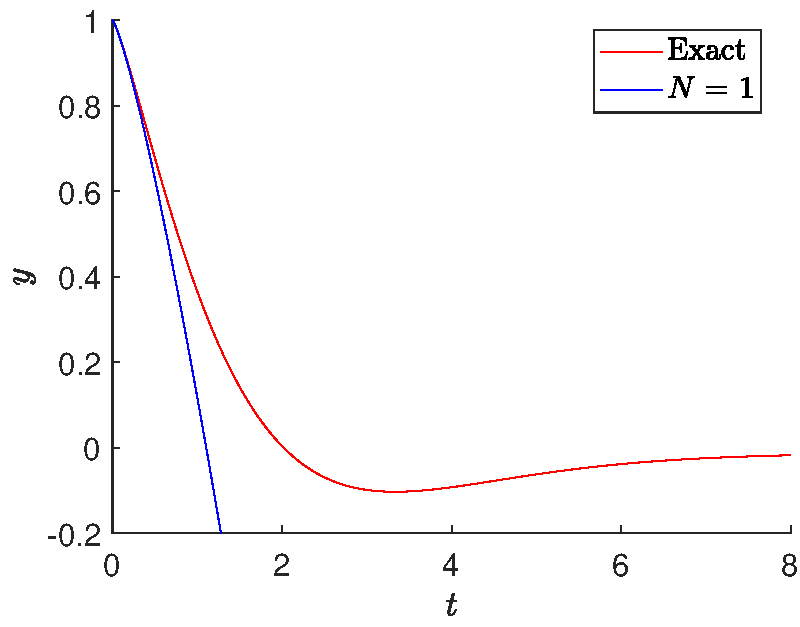
\includegraphics[scale=0.31]{files/comparFrac/Adomian_N_1.pdf}}
        \only<2>{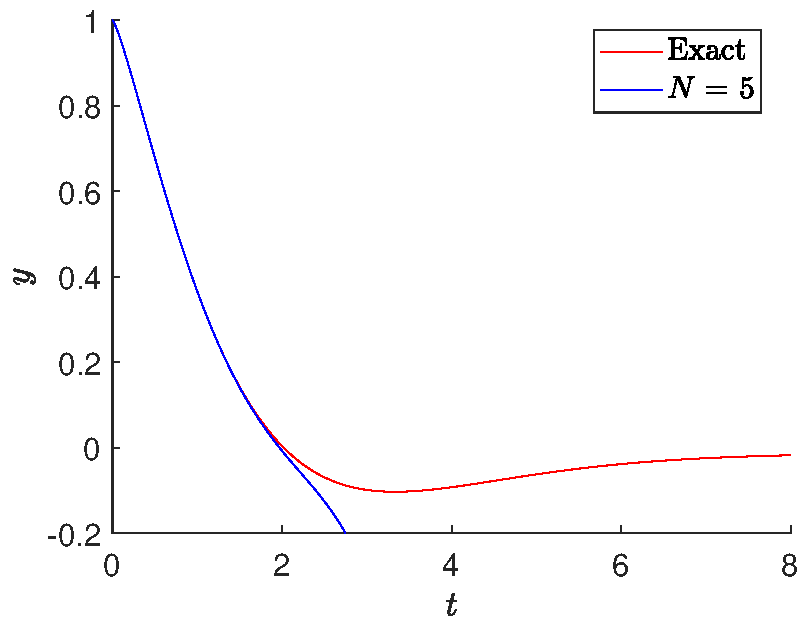
\includegraphics[scale=0.31]{files/comparFrac/Adomian_N_5.pdf}}
        \only<3>{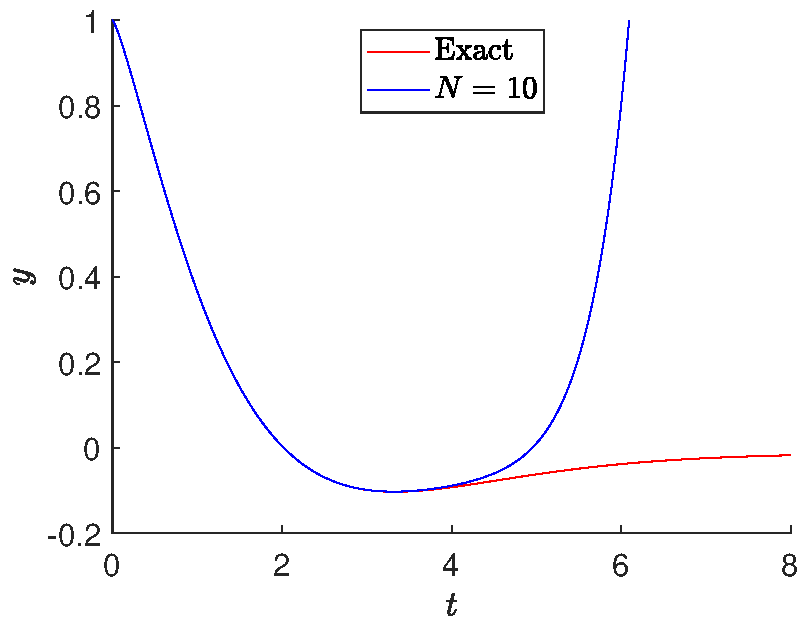
\includegraphics[scale=0.31]{files/comparFrac/Adomian_N_10.pdf}}
        \only<4>{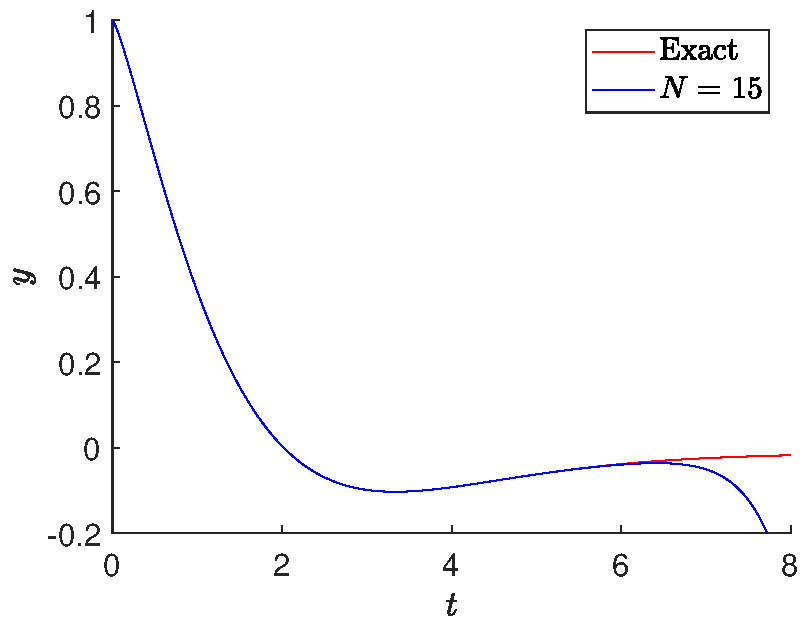
\includegraphics[scale=0.31]{files/comparFrac/Adomian_N_15.pdf}
        }
    \end{figure}
    \end{multicols}
\end{frame}



\subsection{Comparison ABM - Decomposition}
\begin{frame}{FRACTIONAL ORDER METHODS}
\framesubtitle{Comparison ABM - Decomposition}
\begin{equation}
    \begin{cases}
        \dfrac{d^{1.25}}{dt^{1.25}}y(t)=-y(t)&\\
        y'(0)=0,\,y(0)=1
    \end{cases}
\end{equation}

\begin{equation}
    y(t) = E_{1.25,\,1}(-t^{1.25})=\sum_{k=0}^{\infty}\dfrac{(-1)^kt^{1.25k}}{\Gamma(1.25k +1)}
\end{equation}
\begin{multicols}{2}
$\qquad\quad$\textbf{ABM}\begin{figure}[H]
        \centering
        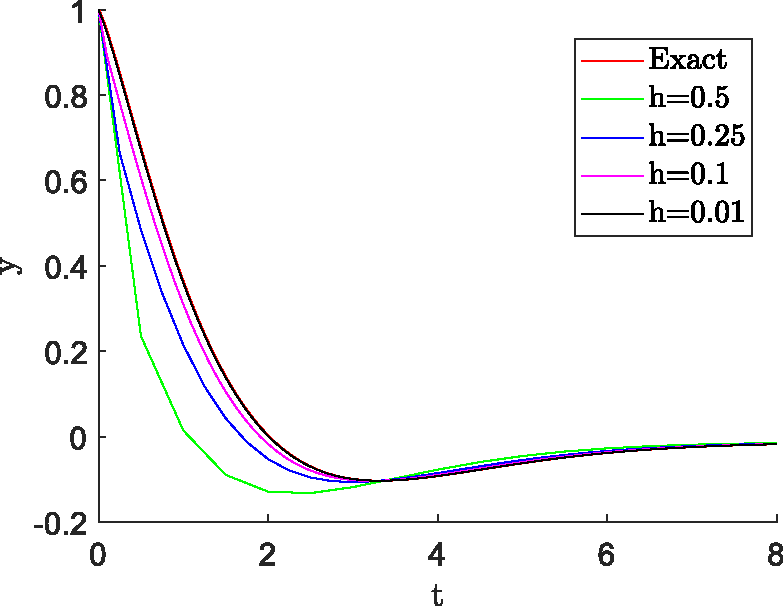
\includegraphics[scale=0.34]{files/ejemplo_adam.pdf}
    \end{figure}\columnbreak$\quad\qquad$\textbf{Decomposition}
    \vspace{-0.5cm}\begin{figure}[H]
        \centering
        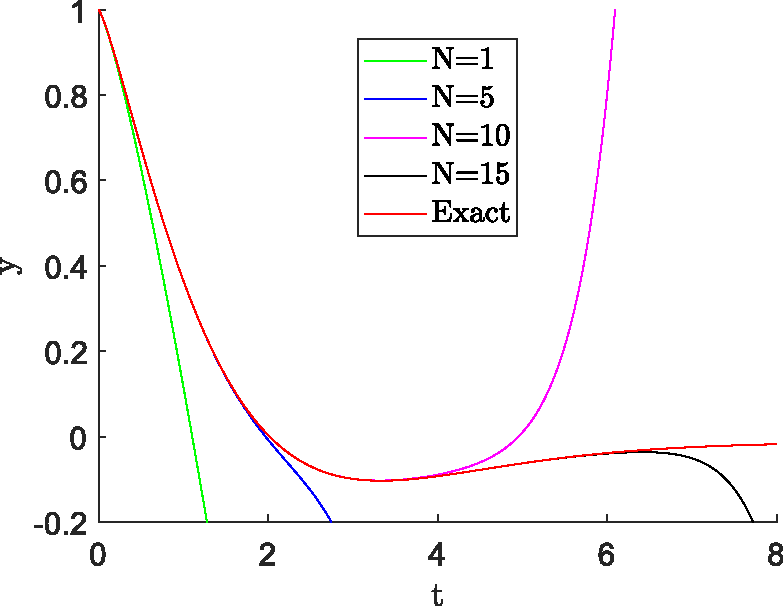
\includegraphics[scale=0.34]{files/frac_deco.pdf}
    \end{figure}
\end{multicols}
\end{frame}

\subsection{Systems of FDEs}
\begin{frame}{FRACTIONAL ORDER METHODS}
    \framesubtitle{Systems of FDEs}
    Consider the system of ordinary fractional differential equations
    \begin{equation}
        \begin{cases}
            \dfrac{d^{\alpha_1}}{dt^{\alpha_1}}y_1=f_1(t,y_1,\,y_2,\,\dots,\,y_n)&y_1(0)=y_{1}\\[6pt] \dfrac{d^{\alpha_2}}{dt^{\alpha_2}}y_2=f_2(t,y_1,\,y_2,\,\dots,\,y_n)&y_2(0)=y_{2}\\
            \qquad\vdots&\\
            \dfrac{d^{\alpha_n}}{dt^{\alpha_n}}y_n=f_n(t,y_1,\,y_2,\,\dots,\,y_n)&y_n(0)=y_{n}\\[6pt]
            \alpha_i\in\mathbb{R}^+,\,\,t\in[0,T]
        \end{cases}
    \end{equation}
    which can be synthesized as 
    \begin{equation}
        \begin{cases}
            \dfrac{d^{\pmb{\alpha}}}{dt^{\pmb{\alpha}}}\mathbf{y}=F(t,\mathbf{y})&\\
            \mathbf{y}(0)=\mathbf{y}_0,\,\pmb{\alpha}\in\left(\mathbb{R}^+\right)^{n\times1},\,t\in[0,T]
        \end{cases}
    \end{equation}
\end{frame}

\subsection{Multi-Term FDEs}
\begin{frame}{FRACTIONAL ORDER METHODS}
\framesubtitle{Multi-Term FDEs}
Suppose we have the multi-term fractional differential equation
\begin{equation}
    \begin{cases}
    \dfrac{d^{\alpha_n}}{dt^{\alpha_n}}y(t)=f\left(t,y,\dfrac{d^{\alpha_{1}}}{dt^{\alpha_{1}}}y,\dfrac{d^{\alpha_{2}}}{dt^{\alpha_{2}}}y,\dots,\dfrac{d^{\alpha_{n-1}}}{dt^{\alpha_{n-1}}}y\right)&\\
    y(0)=y_0,\,\dots,y^{(m-1)}(0)= y_{(m-1)}
    \end{cases}
\end{equation}
    where $m=\ceil{\alpha_n}$ and $0<\alpha_{1}<\alpha_{2}<\ldots<\alpha_{n}$. We select new orders $\tilde{\alpha}_{1}, \ldots, \tilde{\alpha}_{n}$ such that
    \[\begin{array}{l}{\text { (a) } \tilde{\alpha}_{1}, \ldots, \tilde{\alpha}_{n} \text { must be rational numbers, }} \\ {\text { (b) }\left\lceil\alpha_{n}\right\rceil=\left\lceil\tilde{\alpha}_{n}\right\rceil} \\ {\text { (c) } \operatorname{gcd}\left(1, \tilde{\alpha}_{1}, \ldots, \tilde{\alpha}_{n}\right) \text { should be as large as possible, }} \\ {\text { (d) }\left|\alpha_{j}-\tilde{\alpha}_{j}\right| \text { should be as small as possible for all } j}\end{array}\]
\end{frame}


\begin{frame}{FRACTIONAL ORDER METHODS}
\framesubtitle{Multi-Term FDEs}
    We build the approximated system of FDEs with \[\gamma :=\operatorname{gcd}\left(1, \tilde{\alpha}_{1}, \ldots, \tilde{\alpha}_{n}\right)\] 
    \[\tilde{N} :=\frac{\tilde{\alpha}_{n}}{\gamma}\]
    \begin{equation}
    \begin{cases}
    \dfrac{d^{\gamma}}{dt^\gamma} x_{0} =x_{1} &\\[5pt]
    \dfrac{d^{\gamma}}{dt^\gamma} x_{1} =x_{2} &\\
    \qquad\vdots &\\
    \dfrac{d^{\gamma}}{dt^\gamma} x_{\tilde{N}-2} =x_{\tilde{N}-1} &\\[5pt]
    \dfrac{d^{\gamma}}{dt^\gamma} x_{\tilde{N}-1} =f\left(t, x_{0}, x_{\tilde{\alpha}_{1} / \gamma}, \ldots, x_{\tilde{\alpha}_{n-1} / \gamma}\right) \end{cases}
    \end{equation}
    \begin{equation}
    x _ { j } ( 0 ) = \begin{cases} { y _ { ( j \gamma ) }   } & { \text { for } j \gamma \in \mathbb { N } _ { 0 } } \\ { 0  } & { \text { else } } \end{cases}
    \end{equation}
\end{frame}

\begin{frame}{FRACTIONAL ORDER METHODS}
\framesubtitle{Multi-Term FDEs}
    \textbf{Example: Bagley-Torvik Equation} (\href{run:nonNewtonianFluid.gif}{Click for GIF})\\\vspace{0.3cm}
    \begin{equation}
    \begin{cases}
        ay''+b\dfrac{d^{3/2}}{dt^{3/2}}y+cy=g(t)&\\
        y(0)=y_0,\,y'(0)=y_1
    \end{cases}
    \end{equation}
    Let us keep the original orders  $\tilde{\alpha}_1=3/2$ and $\tilde{\alpha}_2=2$ to satisfy condition (d). Note that $\gamma=\operatorname{gcd}(1,3/2,2)=1/2$. Then $\tilde{N}=\dfrac{\tilde{\alpha}_2}{\gamma}=4$. Therefore, the approximated system is
    \begin{equation}
        \begin{cases}
        \dfrac{d^{1/2}}{dt^{1/2}}x_0=x_1&x_0(0)=y_0\\[5pt]
        \dfrac{d^{1/2}}{dt^{1/2}}x_1=x_2&x_1(0)=0\\[5pt]
        \dfrac{d^{1/2}}{dt^{1/2}}x_2=x_3&x_2(0)=y_1\\[5pt]
        \dfrac{d^{1/2}}{dt^{1/2}}x_3=f\left(t,x_0,x_{1.5/0.5}\right)=\dfrac{g(t)-cx_0-bx_3}{a}&x_3(0)=0\\
        \end{cases}
    \end{equation}
\end{frame}

\begin{frame}{FRACTIONAL ORDER METHODS}
\framesubtitle{Multi-Term FDEs}
    \textbf{Example: Bagley-Torvik Equation}\\\vspace{0.5cm}
    In particular, for $a=1$, $b=c=-1$, $g(t)=t+1$, $y_0=1$ and $y_1=1$, the exact solution to this IVP is 
    \begin{equation}
        y(t)=1+t
    \end{equation}
    \begin{figure}[H]
        \centering
        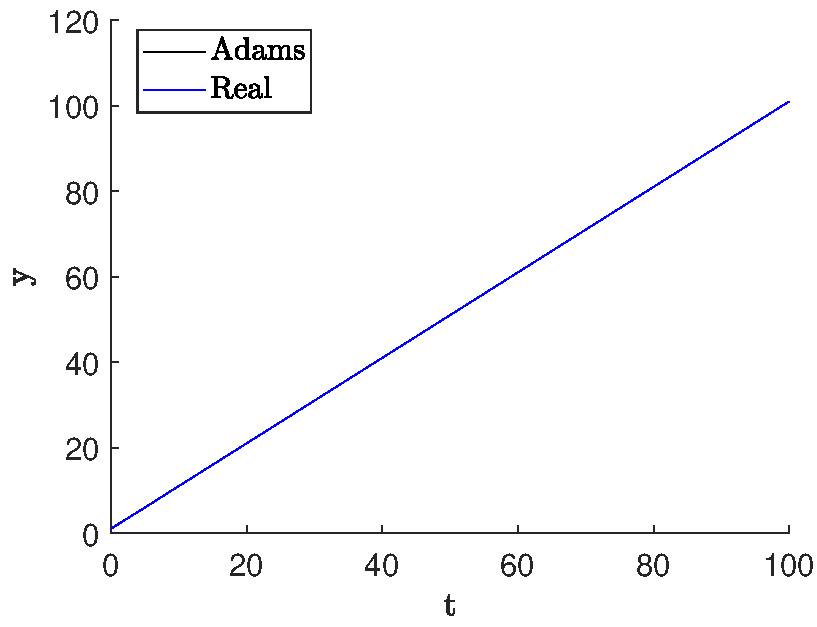
\includegraphics[scale=0.45]{files/abm_system.pdf}
    \end{figure}
\end{frame}






\section{IMPROVEMENTS}
\subsection{Predicted ABM}
\begin{frame}{IMPROVEMENTS}
\framesubtitle{Predicted ABM}
\begin{itemize}
    \item $+$ accuracy $\implies$ $+$ execution time.
    \item ABM converges $\iff$ Predicted ABM converges.
\end{itemize}
    The idea is to calculate different $y _ { h } ^ { \mathrm { p } } \left( t _ { n + 1 } \right)$ until a tolerance is reached, for each instant of time. 
    \begin{center}
    \texttt{y = pabm(f,alpha,y0,T,N,nmax,tol)}
    \end{center}
    For example, using the same Bagley-Torvik equation with larger time step, we have
    \begin{figure}[H]
    \centering
    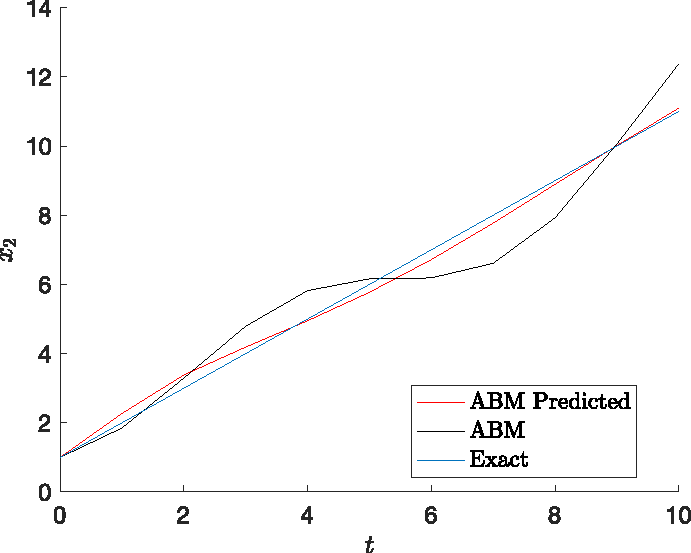
\includegraphics[scale=0.44]{files/mejoras/comparPredictedABM.pdf}
    \caption{Comparison between the original and predicted scheme.}
    \label{fig:comparBagleyTorvik}
\end{figure}
\end{frame}

\subsection{Quadrature Decomposition}
\begin{frame}{IMPROVEMENTS}
\framesubtitle{Quadrature Decomposition}
The idea was to partition the time interval and, on each point, find the polynomial using approximations to the Riemann-Liouville integral.\\[0.4cm]
\begin{center}
    \texttt{y = qDecomposition(f,alpha,y0,N1,N2,T)}
\end{center}
\textbf{Example:}\\[0.4cm]
\begin{multicols}{2}
\begin{equation}
    \begin{cases}
        x'=y&x(0)=1\\
        y'=2x-y&y(0)=-1
    \end{cases}
\end{equation}
\columnbreak
\begin{figure}[H]
    \centering
    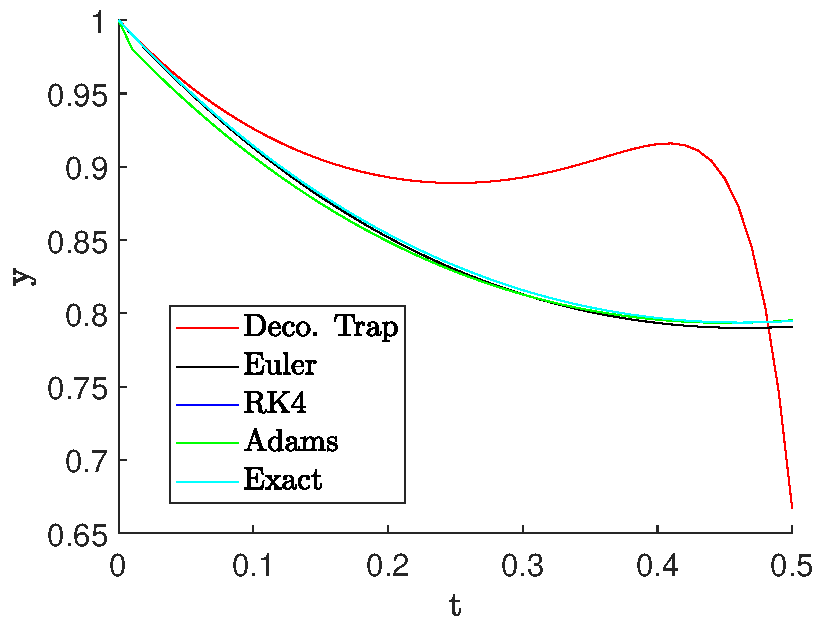
\includegraphics[scale=0.4]{files/mejoras/decom_trap.pdf}
\end{figure}
\end{multicols}
\end{frame}



\subsection{Polynomial Decomposition}
\begin{frame}{IMPROVEMENTS}
\framesubtitle{Polynomial Decomposition}
\begin{itemize}
    \item Analytic solution.
    \item $-$ execution time.
    \item Useful for non-chaotic dynamic systems or chaotic systems for small time frames.
\end{itemize}
The main idea is based on the simple computation of
\begin{equation}
    J^\alpha\left(t^\beta\right)=\dfrac{\Gamma(\beta+1)}{\Gamma(\alpha+\beta+1)}t^{\alpha+\beta}
\end{equation}
which can be extended to non-polynomial expressions using interpolation.

\begin{center}
    \texttt{ySim = pDecomposition(f,alpha,y0,N)}
\end{center}
\end{frame}

\begin{frame}{IMPROVEMENTS}
\framesubtitle{Polynomial Decomposition}
    \textbf{Example:}\\[0.4cm]
    \begin{equation}
        \begin{cases}
        \dfrac{d^3}{dt^3}y(t)+\dfrac{d^{5/2}}{dt^{5/2}}y(t)+y^2(t)=t^4&\\
        y(0)=y'(0)=0,\,y''(0)=2
        \end{cases}
    \end{equation}
    The exact solution is $y(t)=t^2$. Using the procedure for multi-term FDEs, the solution can be approximated as shown in the figure.
    \begin{figure}[H]
        \centering
        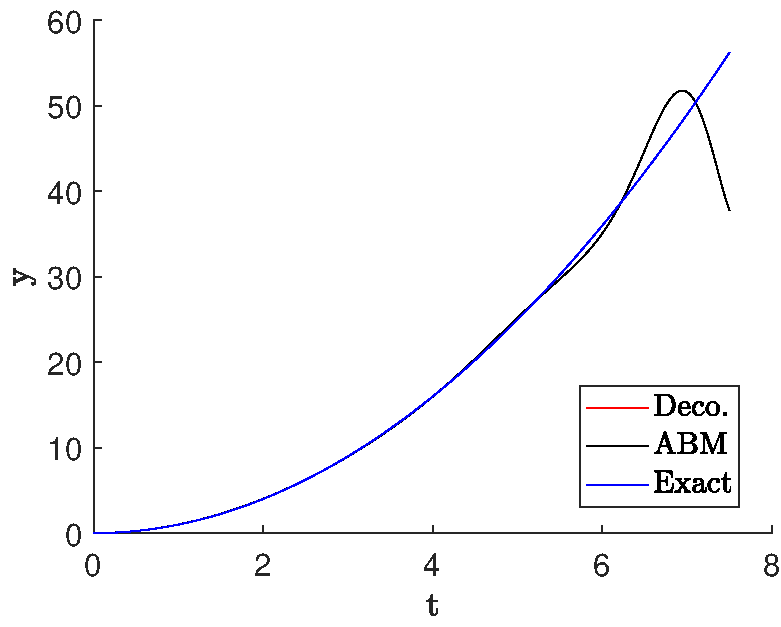
\includegraphics[scale=0.35]{files/mejoras/ABM-vs-Deco-Exact.pdf}
    \end{figure}
\end{frame}

\begin{frame}{IMPROVEMENTS}
\framesubtitle{Polynomial Decomposition}
\textbf{Example: Fractional Lotka-Volterra model}
\begin{equation}
    \begin{cases}{\dfrac{d^{\alpha_1}}{dt^{\alpha_1}}x=\alpha x-\beta x y}& \\[6pt]{\dfrac{d^{\alpha_2}}{dt^{\alpha_2}}y=\delta xy-\gamma y}&\end{cases}
\end{equation}
Using params$=[1,1,1,1]$, c.i$=[1,0.5]$ and $\alpha=[0.5,0.6]$:
\begin{figure}
    \centering
    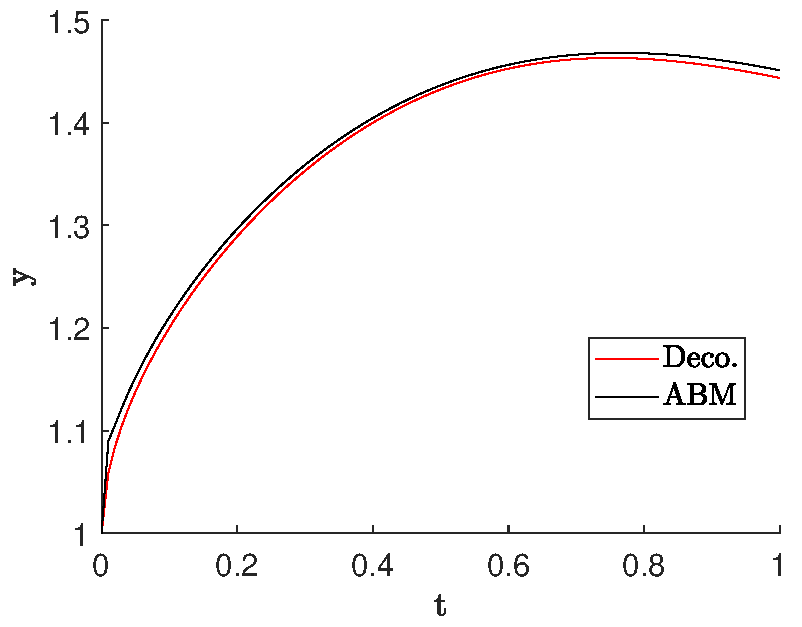
\includegraphics[scale=0.35]{files/mejoras/pred_preey_frac.pdf}
    \end{figure}

\end{frame}

\begin{frame}{IMPROVEMENTS}
\framesubtitle{Polynomial Decomposition}
\textbf{Example: Financial System}
\begin{equation}
    \begin{cases}
    \dfrac{d^{\alpha_1}}{dt^{\alpha_1}} x=z+(y-a)x&\\[6pt]
    \dfrac{d^{\alpha_2}}{dt^{\alpha_2}} y=1-by-x^2&\\[6pt]
    \dfrac{d^{\alpha_3}}{dt^{\alpha_3}} z=-x-cz&
    \end{cases}
\end{equation}
Using params$=[3,0.1,1]$, c.i$=[2,3,2]$ and $\alpha=[1,1,0.8]$, we obtain\begin{multicols}
{2}
\begin{figure}[H]
    \centering
    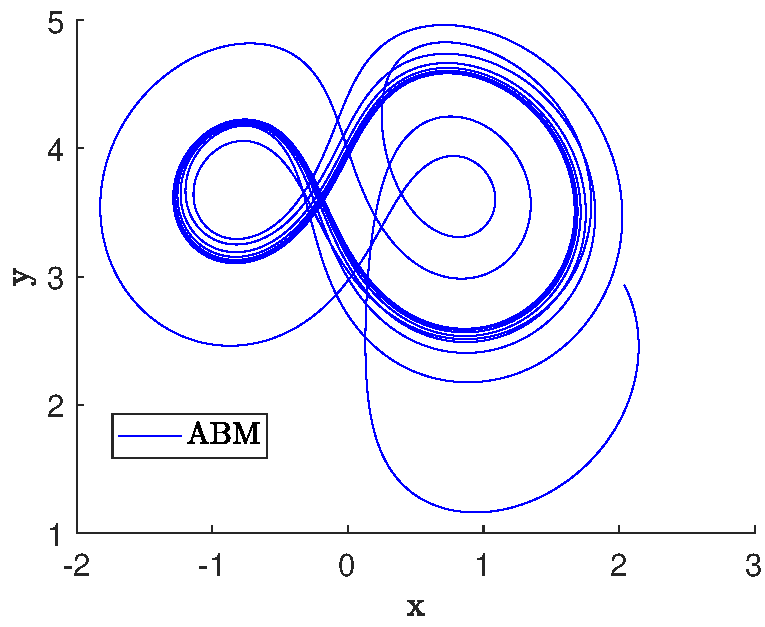
\includegraphics[scale=0.35]{files/comparFrac/finance_chaotic.pdf}
    
\end{figure}
\columnbreak
\begin{figure}[H]
    \centering
    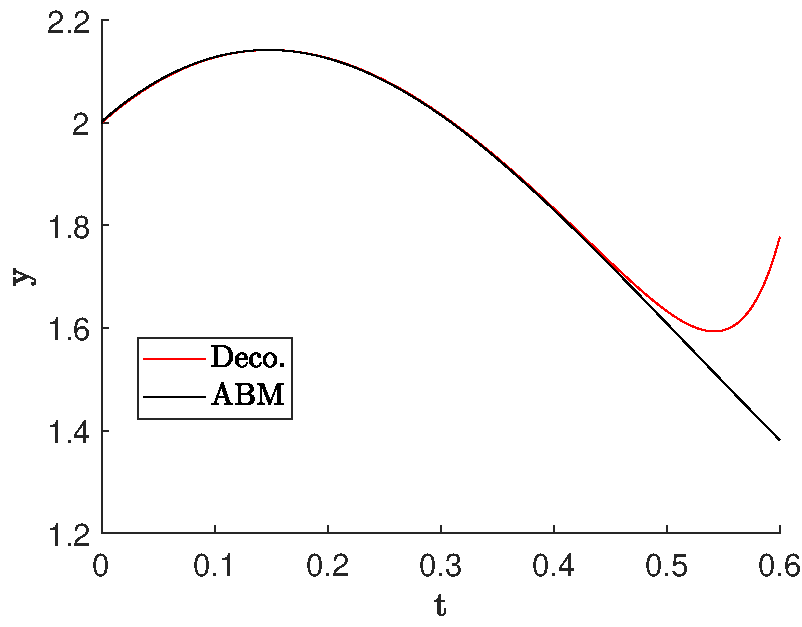
\includegraphics[scale=0.35]{files/mejoras/ABM-vs-Deco-finance.pdf}
\end{figure}
\end{multicols}
\end{frame}

\subsection{Further Work}
\begin{frame}{IMPROVEMENTS}
\framesubtitle{Further Work}
\begin{itemize}
    \item ABM with fixed memory.
    \[\frac { 1 } { \Gamma ( 1 - \alpha ) } \int _ { t - T } ^ { t } \frac { y ^ { \prime } ( s ) } { ( t - s ) ^ { \alpha } } d s\]
    \item ABM with logarithmic memory.
    \[w ^ { p \alpha } \int _ { 0 } ^ { t } \frac { f \left( w ^ { p } x \right) } { ( t - x ) ^ { 1 - \alpha } } d x\]
    \item Richardson extrapolation.
    \[x _ { n } = x \left( t _ { n } \right) + \sum _ { \mu = 1 } ^ { M _ { 1 } } \gamma _ { \mu } n ^ { - \lambda \mu }\]
    \item Decomposition acceleration.
    \[S _ { n } ^ { ( k ) } = \frac { S _ { n } ^ { ( k - 1 ) } S _ { n + 2 } ^ { ( k - 1 ) } - \left( S _ { n + 1 } ^ { ( k - 1 ) } \right) ^ { 2 } } { S _ { n } ^ { ( k - 1 ) } + S _ { n + 2 } ^ { ( k - 1 ) } - 2 S _ { n + 1 } ^ { ( k - 1 ) } } , \quad k \geq 1\]
\end{itemize}
\end{frame}


\section{CONCLUSIONS}
\begin{frame}{CONCLUSIONS}
\begin{multicols}{2}
\begin{itemize}
    \item Fractional calculus $\longrightarrow$ powerful tool to model real and chaotic systems.
    \item Both ABM and decomposition are useful but each with pros and cons.
    \item Both methods can be improved, as shown.
    \item A summary of some essential tools to study fractional systems was successfully constructed.
\end{itemize}
\columnbreak
\begin{figure}[H]
    \centering
    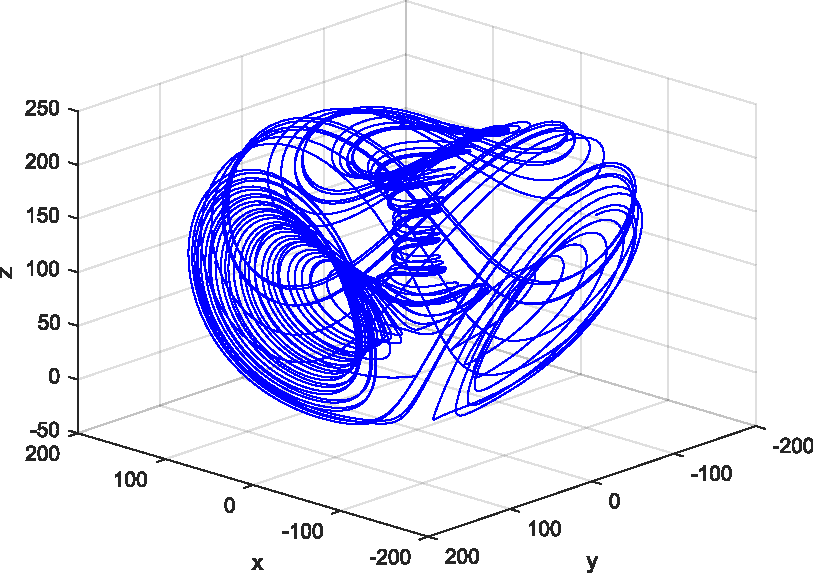
\includegraphics[scale=0.4]{files/3d_chaos.pdf}
\end{figure}
\end{multicols}
\end{frame}
\nonumb
%\addcontentsline{toc}{section}{\small\protect\numberline{}{REFERENCIAS BIBLIOGRÁFICAS}} % Separated from other contents, for small number of contents
\addcontentsline{toc}{section}{\small REFERENCES} % Closer from other contents, for large number of contents
\nocite{*} % All citations showed (take care with fraud!)
%%%%%%%%%%%%%%%%%%%%%%%%%%%%%%%%%%%%%%%%%%%%%%%%%%%%%%%%%%%%%%%%%%%%%%%%%%%%
\section*{REFERENCES}
\begin{frame}[allowframebreaks]{REFERENCES} %  and put before {REFEREN...}
\begingroup % Group for changing the color
\renewcommand{\color}[1]{} % Allows to have black bibs and white footnote bibs
\small{\bibliographystyle{IEEEtran}} % Size of text; acm or gatech-thesis or ieeetr or ieeetran or icontec or iso690
\bibliography{ref}
\endgroup % Group for changing the color
% pdflatex -> bibtex -> pdflatex -> pdflatex
\end{frame}
%%%%%%%%%%%%%%%%%%%%%%%%%%%%%%%%%%%%%%%%%%%%%%%%%%%%%%%%%%%%%%%%%%%%%%%%%%%%
% Thank-slide
\begin{frame}[plain,noframenumbering] % No frame number
	\begin{beamercolorbox}[ht=\paperheight,wd=\paperwidth, center]{Portada}
		\begin{center}\Huge\textbf{Thank you}\end{center} % Or Thanks; leave the next space mandatorily
		
		\vspace{0.44\paperheight}
    \end{beamercolorbox}
\end{frame}
%%%%%%%%%%%%%%%%%%%%%%%%%%%%%%%%%%%%%%%%%%%%%%%%%%%%%%%%%%%%%%%%%%%%%%%%%%%%

\end{document}